\newpage
\subsection{Examples}

\begin{example}[Brauer relation forces growth]
    Let $G = C_2 \times C_6$, with subgroup diagram
    \begin{figure}[H]
        \centering
    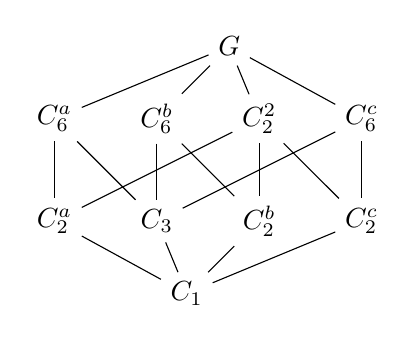
\begin{tikzpicture}[node distance=1.3cm]
        \node(G)[midway]{$G$};
        \node(C6b)[below left of =G]{$C_6^{b}$}; \node(C6a)[left of=C6b]{$C_6^{a}$};  
        \node(C22)[right of=C6b]{$C_2^{2}$};    \node(C6c)[right of=C22]{$C_6^{c}$};
        \node(C2a)[below of=C6a]{$C_2^{a}$};    \node(C3)[below of=C6b]{$C_3$};
        \node(C2b)[below of=C22]{$C_2^{b}$};    \node(C2c)[below of=C6c]{$C_2^{c}$};
        \node(C1)[below left of=C2b]{$C_1$};
        \draw(G)--(C6a);    \draw(G)--(C6b);    \draw(G)--(C6c);    \draw(G)--(C22);
        \draw(C6a)--(C2a);  \draw(C6a)--(C3);
        \draw(C6b)--(C2b);  \draw(C6b)--(C3);
        \draw(C6c)--(C2c);  \draw(C6c)--(C3);
        \draw(C22)--(C2a);  \draw(C22)--(C2b);  \draw(C22)--(C2c);
        \draw(C2a)--(C1);   \draw(C2b)--(C1);   \draw(C2c)--(C1);   \draw(C3)--(C1); 
    \end{tikzpicture}
    \end{figure}
    There is a Brauer relation coming from the $C_2 \times C_2$-quotient, given by $$\Psi = C_3 - C_6^a - C_6^b - C_6^c + 2G.$$ Consider an order $6$ character $\rho_a$ of $G$ with $C_2^{a}$ in its kernel. This has $\bQ(\rho_a) = \bQ(\zeta_6) = \bQ(\zeta_3) = \bQ(\sqrt{-3})$. Then $$\Theta = C_2^{a} - C_6^{a} - C_2^{2} + G$$ is a $\rho_a$-relation, with $\bC[ G / \Theta] = \repnorm{\rho_a}$. 

    Let $E / \bQ$ be a semistable elliptic curve and $F / \bQ$ an abelian extension with $G = \Gal(F / \bQ)$. We claim that $C(\Theta) \in \fieldnorm{\rho_a}$, for all such $E$ (see remark \ref{rephrase-thm}). Since each subgroup in $\Theta$ contains $C_2^{a}$, we have that $C(\Theta)$ equals $C(\Theta / C_2^{a})$ {\color{red} by ref. passing to quotient} where $\Theta / C_2^{a} \in \B(G / C_2^{a}) = \B(C_6)$.  Now $\Theta / C_2^{a}$ is a $\chi_6$-relation, where $\chi_6$ is a faithful order $6$ character of $C_6$. But for cyclic groups we always get norm relations; by Theorem \ref{thm_consistent_cyclic}, $C(\Theta / C_2^{a}) \in \fieldnorm{\chi_a} \implies C(\Theta) \in \fieldnorm{\rho_a}$.

    On the other hand, $C(\Theta + \Psi) = C(\Theta)C(\Psi)$ is not always a norm. Indeed suppose $E / \bQ$ has split multiplicative reduction at a prime $p$ with $D_p = I_p = C_2^{2}$, and any other bad reduction only at unramified primes in $F / \bQ$. Let $\ord_p(\Delta_E) = n$. Then 
        $$C(\Theta) = \frac{2n(4n)^3}{(2n)^3 (4n)} \in \bQ^{\times 2}, \qquad
            C(\Psi) = \frac{n^3(4n)^6}{(2n)^3(2n)^3(2n)^3} = 2 \cdot \square.$$
    Thus $C(\Theta + \Psi) = 2 \mod \bQ^{\times 2}$, but $2$ is not a norm in $\bQ(\sqrt{-3})$. Hence one must have $\rk E / F > 0$. 

    This example shows that we can get different results for different $\rho$-relations. Note that the forced rank growth came from the Brauer relation {\color{red} \ldots}


\end{example}